%\documentclass[journal]{IEEEtran}
\documentclass[12pt, draftcls, onecolumn]{IEEEtran}
\makeatletter
% journal (default) and conference
\def\subsubsection{\@startsection{subsubsection}% name
                                 {3}% level
                                 {\z@}% indent (formerly \parindent)
                                 {0ex plus 0.1ex minus 0.1ex}% before skip
                                 {0ex}% after skip
                                 {\normalfont\normalsize\bfseries}}% style
\makeatother
\usepackage[T1]{fontenc}% optional T1 font encoding
%\usepackage{graphicx}
\usepackage{subfigure}
\usepackage{ulem}
\usepackage{amsmath}
\usepackage{hyperref}
\allowdisplaybreaks
\usepackage{hhline}
\usepackage{yfonts,color}
\usepackage{soul,xcolor}
\usepackage{verbatim}
\usepackage{amsmath}
\allowdisplaybreaks
\usepackage{amssymb}
\usepackage{amsthm}
\usepackage{float}
\usepackage{bm}
\usepackage{url}
\usepackage{array}
\usepackage{cite}
\usepackage{graphicx}
\usepackage{framed} % for frame
\usepackage{balance} % balance
\usepackage{epsfig,epstopdf}
\usepackage{booktabs}
\usepackage{courier}
\usepackage{subfigure}
\usepackage{pseudocode}
\usepackage{enumerate}
\usepackage{algorithm}
\usepackage{algpseudocode}
\newtheorem{definition}{Definition}
\newtheorem{theorem}{Theorem}
\newtheorem{lemma}[theorem]{Lemma}
\newtheorem{proposition}[theorem]{Proposition}
%\newtheorem{proposition}{Proposition}
\newtheorem{corollary}[theorem]{Corollary}
\newtheorem{assumption}{Assumption}
\newtheorem{remark}{Remark}
\renewcommand{\algorithmicrequire}{\textbf{Initialization:}}  % Use Input in the format of Algorithm
\renewcommand{\algorithmicensure}{\textbf{Output:}}  % Use Output in the format of 
\newcommand{\rom}[1]{\uppercase\expandafter{\romannumeral #1\relax}}
\usepackage{color}
\usepackage{soul,xcolor}
\newcommand{\nm}[1]{{\color{blue}\text{\bf{[NM: #1]}}}}
\newcommand{\sst}[1]{\st{#1}}
\newcommand{\gs}[1]{{\color{orange}\bf{[GS: #1]}}}
\newcommand{\remove}[1]{{\color{magenta}{\bf REMOVE: [#1]}}}
%\newcommand{\nm}[1]{}
%\newcommand{\sst}[1]{}
%\newcommand{\gs}[1]{}
%\newcommand{\remove}[1]{}
\newcommand{\add}[1]{{\color{red}{#1}}}
\newcommand{\ull}[1]{\textbf{\color{red}\ul{#1}}}
%\pagestyle{empty}
\normalem
\begin{document} 
\setulcolor{red}
\setul{red}{2pt}
\title{Cross-Layer Optimization in Decentralized Cognitive Radio Networks}
\author{Bharath Keshavamurthy}
\maketitle
\setstcolor{red}
\begin{abstract}
In the cognitive radio networks paradigm, unlicensed users termed as Secondary Users (SUs) need to learn to co-exist with licensed users termed as Primary Users (PUs) while ensuring strict non-interference with the incumbent transmissions and at the same time provide certain QoS guarantees such as maximum allowed latency and minimum sustained throughput for the flows allotted to them. In this regard, the design of the SU network stack is influenced by the spectrum access protocols implemented in the MAC layer. However, pure divide-and-conquer strategies such as developing and incorporating a new MAC layer scheme for channel access while leaving the conventional network protocols in the other layers of the SU stack untouched do not work due to the various dependencies across all the layers of the stack. Considering this, we present a cross-layer optimization framework that captures the design novelty and inter-layer dependence needed in order to tackle the additional requirement of co-existence with incumbents and the other cognitive radio nodes. We take the convex optimization route to solve for the optimal protocols to be employed in the various layers of the SU network stack - formulate a utility maximization problem with numerous constraints that capture the QoS requirements, power allocation restrictions, MCS adaptation features, flow rate requirements, prioritized flow handling, and non-interference compliance; decouple the global, integrated, cross-layer optimization problem using decomposition techniques; and solve these decoupled sub-problems using tools from standard Lagrangian duality theory, descent methods, and custom heuristic algorithms. Additionally, assuming a Markovian correlation model in the occupancy behavior of the incumbents both spatially and temporally, we present parameter estimation techniques to learn the correlation model, state estimation techniques to estimate the occupancy states, and a POMDP agent to learn the occupancy behavior over time by interacting with the radio environment and assign availability/utility metrics to channels which are then integrated into the derived CSMA protocol's back-off timer logic at the MAC layer of the SU network protocol stack.
\end{abstract}
\newpage
%%%%%%%%%% Introduction %%%%%%%%%%
\section{Introduction}
\subsection{Motivation - Why Cross-Layer Optimization?}
\begin{itemize}
  \item Objective: Maximize the throughput of a set of assigned end-to-end multi-hop flows in a Secondary User (SU) network by intelligently exploiting the spectrum holes left unused by the licensed user
  \item Pure divide-and-conquer protocol design strategies do not work because the performance across all layers are dependent on the resource allocation constraints and the incumbent interference constraints.
  \item A cross-layer optimization framework is the way-to-go because it brings in requirements from all five layers of the stack with one global objective of maximizing the throughput while enforcing strict non-interference compliance with the incumbent transmissions.
  \item Devise a distributed, layered solution for the optimal performance of a cognitive radio node
\end{itemize}
\subsection{Objectives and contributions}
The objective of this project is to develop joint flow control, prioritized flow scheduling, spectrum allocation, MCS adaptation, and transmission power control techniques for Secondary Users in decentralized cognitive radio networks with QoS guarantees. We present a five-layer optimization strategy for the design of the SU network protocol stack in Cognitive Radio Ad-Hoc Networks (CRAHNs) otherwise known as decentralized cognitive radio networks.
\\The main contributions of this project are detailed below:
\begin{itemize}
    \item Formulate a Numerical Utility Maximization (NUM) optimization problem with constraints that capture all the critical design aspects of the SU network protocol stack such as transmission power control, MCS adaptation, spectrum access, prioritized flow scheduling, and flow rate control - all these aspects are designed with the primary goal of meeting the QoS requirements guaranteed by services in the application layer while ensuring the SUs do not interfere with the incumbent transmissions
    \item Fragment this complex, joint, cross-layer optimization problem into several sub-problems using Vertical Decomposition techniques
    \item The sub-problems are then solved using standard convex optimization techniques which include Lagrangian \& dual formulations and sub-gradient projection to arrive at the optimal algorithms to be employed in the various layers of the SU network protocol stack
    \item MCS adaptation in the PHY - Frame it as an optimization problem and incorporate it into the cross-layer framework
    \item An intelligent, process-interactive agent model to learn the channel occupancy behavior of the incumbents
    \item The incumbent channel occupancy behavior is not independent spatially and temporally - there exists a correlation model
    \item Different flows have different QoS constraints and hence, some flows need to be prioritized over others - weighted flow scheduling
    \item Assuming a Markovian correlation in the occupancy behavior both spatially and temporally, separate correlation model problems are formulated and solved in order to learn the model and estimate the occupancy states of the channels from noisy and incomplete observations
    \item A POMDP agent is formulated which interacts with the radio environment to arrive at an optimal policy based on the ``belief" of the system state. Standard value iteration techniques cannot be employed to solve for the optimal policy of the POMDP due to the inherent computational complexity. Instead, we employ a randomized point-based value iteration algorithm called the PERSEUS algorithm to solve for an approximate solution to the optimal policy of the POMDP agent. The results from the optimal policy run are integrated into the MAC-layer protocol via the channel utility metrics.
    \item The nodes in the implementation architecture outlined in this paper do not perform any explicit optimization. Instead, by locally executing the Network Protocols arrived at theoretically, which include the queue differential back-pressure scheduler and the modified CSMA algorithm at the nodes, the SU network achieves the QoS requirements guaranteed by the services in the application layer, i.e. the minimum throughput requirements for the multi-hop flows while ensuring that the interference with the licensed user is kept to a minimum.
    \item Also, the system architecture relies on the SUs exchanging their queue lengths over a common control channel. Furthermore, the global quorum-designated gateway node shares the optimal policy statistics, i.e. the channel utility metrics in each time-slot to all the SUs in the network over the common control channel.
\end{itemize}
\clearpage
\section{Related Work}
\begin{itemize}
  \item Y. Teng and M. Song, ``\href{http://ieeexplore.ieee.org/stamp/stamp.jsp?tp=&arnumber=7859326&isnumber=7859429}{\textcolor{blue}{Cross-Layer Optimization and Protocol Analysis for Cognitive Ad Hoc Communications}}"
  \begin{itemize}
      \item Power Allocation, Channel Allocation, Routing, and Flow Rate Control solutions with MRR in the APP - GUOP formulations
      \item Convex optimization using vertical decomposition techniques (COVD)
      \item Complexity analysis and heuristics to overcome the computational overhead/intractability (COHA)
      \item Assumes an independent channel occupancy model, i.e. the occupancy behavior of the incumbent in the network is independent across channels
      \item Assumes that the PU occupancy behavior is known to all the SUs apriori
      \item Standard unit-flows are assumed
      \item MCS adaptation is not considered
      \item Incorporates the idea of a channel stability metric using the concept of Spectrum Life-Time (SLT) - this enables the nodes to perceive the utility of a channel based on its stability instead of relying purely on the observations of occupancy at a given time
  \end{itemize}
  \item A. Cammarano, F. L. Presti, G. Maselli, L. Pescosolido and C. Petrioli, ``\href{http://ieeexplore.ieee.org/stamp/stamp.jsp?tp=&arnumber=6881740&isnumber=7180482}{\textcolor{blue}{Throughput-Optimal Cross-Layer Design for Cognitive Radio Ad Hoc Networks}}"
  \begin{itemize}
      \item MAC, Rate Control, and Flow Scheduling - NUM problem formulation
      \item MCS adaptation is not considered in this problem
      \item Assumes that all the SUs in the network know the occupancy behavior of the incumbents apriori
      \item Standard unit-flows are assumed
      \item Common control channel for the dissemination of known channel occupancy behavior and queue lengths at links for different flows
      \item A static multi-graph topology for the SU network and a conflict graph to capture scheduling constraints among sub-links
      \item Modelling the interference with PUs and other SUs in the network as a conflict graph and scheduling only those links (nodes of the graph) which do not have an edge (conflict in the real-world) between them
      \item Introduction of Wireless Spectrum Sensor Networks (WSSNs) wherein spectrum sensors co-located with the SUs are employed to off-load the sensing capabilities of the SUs thereby, to an extent, simplify the development process
      \item The back-off timer logic in the modified CSMA protocol is highly intuitive - higher the back-pressure on the queues of the links ($q_{h(l)f} - q_{t(l)f}$) and greater the channel availability (captured by $\alpha_{(n,m;c)}$), the shorter are the back-off times (captured by $R_{(n,m;c)}$) and hence, the nodes follow a more aggressive channel access strategy and vice-versa.
  \end{itemize}
  \item Kaelbling, et. al, ``\href{https://people.csail.mit.edu/lpk/papers/aij98-pomdp.pdf}{\textcolor{blue}{Planning and acting in partially observable stochastic domains}}" 
  \\This work details a few Exact Value Iteration algorithms to solve for the optimal policy in POMDPs.
    \begin{itemize}
        \item Given a set of policy trees $\Bar{\nu}$, the authors defines a unique minimal subset of $\Bar{\nu}$ denoted $\nu$ called a parsimonious representation of the value function and a policy tree is deemed useful if it's a part of this parsimonious representation of the value function.
        \item To construct the parsimonious representation of the value function, the Exhaustive Enumeration strategy involves two phases: Generation and Pruning. The generation phase involves constructing a larger representation of $\nu_t$ denoted by $\nu_t^+$ from $\nu_{t-1}$, the set of useful $(t-1)$-step policy trees while the pruning phase requires one linear program for each element of the starting set of policy trees to produce the parsimonious representation of $V_t$.
        \item The Exhaustive Enumeration strategy is exponential in the observation space, i.e. $|\mathcal{A}||\nu_{t-1}|^{|\Omega|}$. So, the authors propose the Witness Algorithm.
        \item The Witness Algorithm avoids generating $\nu_t^+$, instead computes the elements of $\nu_t$ directly. The Witness Algorithm involves computing for each action $a$, a set $Q_t^a$ of $t$-step policy trees that have $a$ at the root, taking a union of all the $Q_t^a$ sets for all actions, and then pruning it to obtain $\nu_t$.
        \item However, the Witness Algorithm is untenable for problems with continuous observation spaces, large state spaces, and hence, large belief spaces.
    \end{itemize}
    \item Spaan and Vlassis, ``\href{https://people.csail.mit.edu/lpk/papers/aij98-pomdp.pdf}{\textcolor{blue}{Perseus: Randomized Point-based Value Iteration for POMDPs}}"
    \\This work details a few Approximate Value Iteration algorithms to solve for the optimal policy in computationally expensive POMDP problems.
    \begin{itemize}
        \item The Exact Value Iteration Algorithms are generally intractable for large problems because these algorithms involve determining the optimal action for every belief in the belief space $\mathcal{B}$.
        \item Instead, for large problems, a more prudent approach would be to perform the backup procedure only over a set of "reachable beliefs". It is shown here that approximate point-based methods which perform backup steps over a reduced set of so-called "reachable beliefs" can find successful policies for the POMDP.
        \item One approach would be the Point-Based Value Iteration (PBVI) Algorithm which involves the following steps:
        \begin{itemize}
            \item Start with a small set of beliefs $B_0$ and perform a series of backups on $B_0$
            \item Expand $B_0$ to $B_1$ by sampling more beliefs. Arbitrarily speaking, the belief set $B_t$ is expanded to $B_{t+1}$ by simulating actions for all $b \in B_t$ and keeping only the belief points that are the farthest away from the points already in $B_{t+1}$
            \item The algorithm then performs a series of backups on $B_{t+1}$ and then expands it to $B_{t+2}$ by employing the "farthest-distance sampling" approach. This continues until a satisfactory condition is reached or until the computation time expires.
        \end{itemize}
        \item The problem with the PBVI Algorithm is that it involves computing the distance between all $b \in B_t$ and furthermore, it also involves backing-up on all $b \in B_t$ generating $|B_t|$ vectors. This may turn out to be computationally expensive or intractable for problems requiring large $|B_t|$.
        \item Another approach which would solve the problems encountered by the PBVI algorithm is the PERSEUS algorithm. The PERSEUS algorithm does not involve computing distances between all belief points in $B_t$ and furthermore, it does not involve performing backups on all $b \in B_t$. Instead, the PERSEUS algorithm involves backing-up only on a subset of $B_t$ while ensuring that the computed solution is effective for the entire set $B_t$.
        \item By performing backups only on a subset of $B_t$ while ensuring optimality/near-optimality for the entire set $B_t$ curbs the increase in the number of vectors as the algorithm progresses.
    \end{itemize}
\end{itemize}
\clearpage
\section{Detailed Description of the Models}
\subsection{The Secondary Network Model}
We model the SU Network as a static multigraph with $N$ nodes and $L$ links - more concisely represented by,
\[\mathcal{G} \triangleq\ (\mathcal{N},\ \mathcal{L})\] 
where,
\\$\mathcal{N}\ =\ \{1,\ 2,\ 3,\ ...,\ N\}$ constitutes the set of secondary users (nodes in the multigraph)
\\$\mathcal{L}\ =\ \{(n,\ m;\ c),\ n,\ m \in \mathcal{N}, c \in \mathcal{C}\}$ constitutes the set of all links in the network (edges of the multigraph) with $n\ =\ h(l)$ as the head of the link, $m\ =\ t(l)$ as the tail of the link, and $c\ =\ c(l)$ as the channel used by the link
\\where, 
\\$C\ =\ \{c_1,\ c_2,\ c_3,\ ...,\ c_K\}$ constitutes the set of channels in our wideband spectrum of interest, each of bandwidth $B$ and capacity $C$ (given by the standard capacity equation).
\\The existence of the link $(n,\ m;\ c)$ means that node $n$ can communicate with node $m$ using channel $c$.
\\For each node $n \in \mathcal{N}$, we define the set of incoming links as,
\[\mathcal{L}_i(n)\ \triangleq\ \{l\ =\ (m,\ n';\ c) \in \mathcal{L}:\ n'\ =\ n\}\]
And the set of outgoing links as,
\[\mathcal{L}_o(n)\ \triangleq\ \{l\ =\ (n',\ m;\ c) \in \mathcal{L}:\ n'\ =\ n\}\]
We also assume that periodic updates of the availability of the channels in the wideband spectrum of interest are sent over to all the SUs in the CRAHN and these SUs occupy spectrum holes identified from this information. Based on this obtained channel availability information, each SU, i.e. $n \in \mathcal{N}$ computes, for each of its outgoing links $(n,\ m)$ a set of channel availability coefficients denoted by $\alpha_{(n,\ m;\ c_1)},\ \alpha_{(n,\ m;\ c_2)},\ \alpha_{(n,\ m;\ c_3)},\ ...,\ \alpha_{(n,\ m;\ c_K)}$. These channel availability coefficients combine the belief that channel $c \in \mathcal{C}$ is free in the nominal interference region of the SU along with the availability of node $m$ to receive on this specific channel. The availability information is contained in the periodic updates sent out by the gateway node. The gateway node consists of a POMDP agent that interacts with the environment and comes up with an interpretation of channel availability which is then shared with other SUs in the network over the common control channel.
\\For sub-link $l \in \mathcal{L}$, we define the channel fading coefficient as $g_l$.
\\Let the power allocated to SU $n$ on channel $c$ and link $l = (n,m;c)$ for flow session $f$ be denoted as $P_{n,l}^f$ while the maximum power budget for user $n \in \mathcal{N}$ is $P_n^{max}$.
\\Now, consider the link adaptation model described below.
We impose a constraint on the maximum allowed Packet Error Rate (PER) as,
\[\mathbb{P}(PER_{MCS} > PER_{allowed}) \leq 0.05\]
\[PER = f(\sigma_V^2,\ MCS-choice,\ G,\ L)\]
In other words, the PER is a function of the noise variance $\sigma_V^2$, the choice of MCS, the channel realization $G$, and the packet length.
We employ a receiver-based MCS selection strategy as described in the subsequent sections of this document. We also assume that all the symbols in the packet experience approximately the same channel.
\subsection{The Traffic Model}
Let, $\mathcal{F}\ \triangleq\ $The set of all end-to-end flows in the CRAHN with weights $w_f$, and,
\\$(s(f),\ d(f)) \in \mathcal{N}^2\ \triangleq\ $the <src, dst> node pair associated with the flow $f \in \mathcal{F}$
\\where, $s(f),\ d(f) \in \mathcal{N}$.
\\Let $x_f$ be defined as the average number of bits/second produced by the source node $s(f)$.
\\We now pose non-negative and maximum flow rate constraints for $x_f$ as shown below.
\[x_f \in [0,\ x_M]\]
We also pose the node balance equations for the flows as follows,
\begin{equation*}
    \begin{cases}
        x_f + \sum_{l \in \mathcal{L}_i(n)}\ s_{fl}\ =\ \sum_{l \in \mathcal{L}_o(n)}\ s_{fl}, & \text{if}\ n\ =\ s_{f},\ f \in \mathcal{F}\\
        \sum_{l \in \mathcal{L}_i(n)}\ s_{fl}\ =\ \sum_{l \in \mathcal{L}_o(n)}\ s_{fl}, & \text{if}\ n\ \not=\ s_{f},\ d_f,\ f \in \mathcal{F}
    \end{cases}
\end{equation*}
Each flow $f \in \mathcal{F}$ is associated with a utility function $U_f(x_f)$ which is assumed to be strictly concave, non-decreasing, and differentiable. We use the utility function given by $\frac{x_f^{1-\eta}}{1-\eta},\ \eta > 0$.
\subsection{The Interference/Conflicts Model}
The following are some of the key design aspects of the Interference Model used in our design.
\begin{enumerate}
    \item Co-Channel Interference: The sender of one link is in the interference range of the sender or the receiver of another link and both links use the same channel
    \item Owing to the physical design constraints of the SU nodes, it's assumed that each node can transmit over only one channel at a given time. Therefore, it is important to note that for a given SU $n \in \mathcal{N}$, link $l \in \mathcal{L}_o(n)$ has conflicts with other outgoing links of the node, i.e. $l' \in \mathcal{L}_o(n)$ where, $l\ \not=\ l'$ and $c(l)\ \not=\ c(l')$.
    \item In order to efficiently capture these conflicts, we employ a {Conflict Graph} denoted by $\mathcal{G}_C\ =\ (\nu,\ \epsilon)$, wherein the nodes of the graph ($\nu$) represent the links and the edges in the graph ($\epsilon$) represent the conflicts between the links. So, intuitively, two links cannot transmit over the same channel at the same time if there is an edge between them.
    \item Let, $\mathcal{I}\ \subseteq\ \nu$ be the collection of sets of links in the network which can transmit at the same time without conflicts/interference with each other. These are also termed as the independent sets of $\mathcal{G}_c$.
    \item $I \in \mathcal{I}$ is a binary vector indicating which links belong to that independent set represented by $I$. In other words, $I\ =\ [a_{I1},\ a_{I2},\ a_{I3},\ ...,\ a_{IL}]$ where, $a_{Il}\ =\ 1$, if $l \in I$ and $a_{Il}\ =\ 0$, if $l \not\in I$.
    \item $p_I$ is defined as the frequency with which the set $I \in \mathcal{I}$ is scheduled such that $\sum_{I \in \mathcal{I}}\ p_I\ =\ 1$.
    \item From the above points, we obtain an expression for the average transmission rate over a link $l$ as,
    \[\sum_{f \in \mathcal{F}}\ s_{fl}\ =\ \sum_{I \in \mathcal{I}}\ p_I a_{Il}\]
\end{enumerate}
We now discuss the model for the evaluation of channel availability metrics in each time-slot using a POMDP agent. The output of the agent fits into the cross-layer optimization's MAC protocol through the aforementioned availability metrics $\alpha$.
\subsection{The Observation Model}
We consider a network consisting of one licensed user termed the Primary User (PU) and one cognitive radio node termed the Secondary User (SU) which is equipped with a spectrum sensor. The SU should learn to intelligently access spectrum holes (white-spaces) in order to maximize its throughput while maintaining strict non-interference compliance with incumbent transmissions. The wideband signal observed at the SU receiver is denoted as $y(n)$ and is given by,
\begin{equation}\label{1}
    y(n)\ =\ \sum_{m=0}^{M-1} h(m)x(n-m) + v(n)
\end{equation}
Here, $y(n)$ is expressed as a convolution of the PU signal $x(n)$ with the channel impulse response $h(n)$, added with a noise term v(n).
Equation (\ref{1}) can be written in the frequency domain by taking a K-point DFT which decomposes the observed wideband signal into K discrete narrow-band components as shown below,
\begin{equation}\label{2}
    Y_k(i)\ =\ H_kX_k(i) + V_k(i)
\end{equation}
where,
\\$i \in \{1,2,3,...,T\}$ represents the index of the observation
\\$k \in \{1,2,3,...,K\}$ represents the index of the channel
\\$V_k(i) \sim \mathcal{CN}(0,\sigma_V^2)$ represents the circular symmetric additive complex Gaussian noise sample i.i.d across channel indices and across time indices. These noise samples are assumed to be independent of the occupancy state of the channels.
\\$H_k \sim \mathcal{CN}(0,\sigma_H^2)$ represents the $k^{th}$ DFT coefficient of the impulse response $h(n)$ of the channel in between the PU and the SU receiver; we model it as a zero-mean circular symmetric complex Gaussian random variable with variance $\sigma_H^2$. These impulse response samples are assumed to be independent of the occupancy state of the channels. The PU occupancy behavior in each sub-band is modelled as $X_k \in \{0,1\}$ taking two possible values $0\ (Idle)$ and $1\ (Occupied)$. Therefore, the PU occupancy behavior in the entire wideband spectrum of interest discretized into narrow-band frequency components at time index $i$ can be modelled as a vector as shown below.
\begin{equation}\label{3}
    \vec{X}(i)\ =\ [X_1(i),X_2(i),X_3(i),...,X_K(i)]^T \in \{0,1\}^K
\end{equation}
\subsection{The Correlation Model}
We model the spectrum occupancy dynamics as a Markov process with the following transition model. Given $\vec{X}(i)$, the spectrum occupancy state at time index $i$, $\vec{X}(i+1)$ is independent of the past, $\vec{X}(j),\ j < i$; $j, i \in \{1,2,3,...,T\}$, i.e.
\begin{equation}\label{4}
    \begin{aligned}
        \mathbb{P}(\vec{X}(i+1)|\vec{X}(j),\ \forall j \leq i)\ =\ \mathbb{P}(\vec{X}(i+1)|\vec{X}(i))
    \end{aligned}
\end{equation}
Additionally, the spectrum occupancy vector $\vec{X}(i)$ exhibits Markovian correlation across the sub-bands as,
\begin{equation}\label{5}
    \begin{aligned}
         \mathbb{P}(\vec{X}(i+1)|\vec{X}(i))\ =\ 
         \prod_{k=1}^K\ \mathbb{P}(X_{k+1}(i+1)|X_{k+1}(i),X_{k}(i))
    \end{aligned}
\end{equation}
The true states encapsulate the actual occupancy behavior of the PU and the measurements at the SU are noisy observations of these true states which are modelled to be the observed states of a Hidden Markov Model. Owing to physical design limitations at the SU's spectrum sensor, not all sub-bands in the discretized spectrum can be sensed. Given this constraint, we model the emission process of the HMM as shown below.
\\The observation vector at time index $i$ is given by,
\begin{equation}\label{6}
    \vec{Y}(i)\ =\ [y_1(i),y_2(i),\phi,y_4(i),...,\phi,y_{K-1}(i),y_K(i)]^T
\end{equation}
where, $y_k(i) = \phi$ indicates that the SU did not sense sub-band $k$ at time index $i$. Therefore, the observation probability termed as the emission probability of the HMM is given by,
\begin{equation*}
    m_r(y_k(i)) \triangleq \mathbb{P}(y_k(i)|x_k(i)=r)
\end{equation*}
where,
\begin{equation}\label{7}
    \begin{aligned}
        m_r(y_k(i))\ &\sim \mathcal{CN}(0,\sigma_H^2r+\sigma_V^2),\ \text{if $y_k(i) \not = \phi$} \\
        m_r(y_k(i))\ &=\ 1,\ \text{if $y_k(i) = \phi$}
    \end{aligned}
\end{equation}
Now, we model the spectrum access scheme of the SU as a Partially Observable Markov Decision Process (POMDP) wherein the goal of the POMDP agent is to devise an optimal sensing and access policy in order to maximize its throughput while maintaining strict non-interference compliance with incumbent transmissions.
\subsection{The POMDP Agent Model}
The agent's limited observational capabilities coupled with its noisy observations result in an increased level of uncertainty at the agent's end about the occupancy state of the spectrum under consideration and the exact effect of executing an action on the radio environment. The transition model of the underlying MDP as described in the Correlation Model of this paper, is denoted by $A$ and is learnt by the agent by interacting with the radio environment. The emission model $B$ is given by (\ref{7}).
We model the POMDP as a tuple $(\mathcal{X},\mathcal{A},\mathcal{Y},\mathcal{B},A,B)$ where, $\mathcal{X}$ represents the state space of the underlying MDP with states $\vec{x}$ which are realizations of the spectrum occupancy vector as given by (\ref{3}) and $|\mathcal{X}|=2^K$, $\mathcal{A}$ represents the action space of the agent considering the imposed sensing limitations, $\mathcal{Y}$ represents the observation space of the agent based on the Observation Model outlined earlier in the paper, and $\mathcal{B}$ represents the belief space of the agent.
\\The run-time or interaction time of the agent is quantized into discrete time-steps termed as episodes. At the beginning of each episode, the agent executes an action $a \in \mathcal{A}$, observes $\vec{y} \in \mathcal{Y}$, and updates it belief $\forall \vec{x}'$ as follows.
\begin{equation}\label{8}
    \begin{aligned}
        b_a^{\vec{y}}(\vec{x}')\ =\ \mathbb{P}(\vec{x}'|\vec{y},a,\vec{b})\ =\ \frac{\mathbb{P}(\vec{y}|\vec{x}',a)}{\mathbb{P}(\vec{y}|a,\vec{b})}\sum_{\vec{x} \in \mathcal{X}}\mathbb{P}(\vec{x}'|\vec{x},a)b(\vec{x})
    \end{aligned}
\end{equation}
where, $\mathbb{P}(\vec{y}|a,\vec{b})$ is the normalization constant given by,
\begin{equation}\label{9}
        \mathbb{P}(\vec{y}|a,\vec{b})\ =\ \sum_{\vec{x}' \in \mathcal{X}}\mathbb{P}(\vec{y}|\vec{x}',a)\sum_{\vec{x} \in \mathcal{X}}\mathbb{P}(\vec{x}'|\vec{x},a)b(\vec{x})
\end{equation}
$\vec{b} \in \mathcal{B}$ represents the belief vector of the agent, i.e. a probability distribution over all states, in the previous time-step,
$b(\vec{x}) \in \vec{b}$ is termed the belief and it represents the degree of certainty assigned to world state $\vec{x} \in \mathcal{X}$ by the belief vector $\vec{b}$. The belief, by definition being a probability measure, has to satisfy the Kolmogorov's axioms, i.e.
\begin{equation}\label{10}
    \begin{aligned}
        \sum_{\vec{x} \in \mathcal{X}} b(\vec{x})\ &=\ 1 \\
        0 \leq b(\vec{x}) &\leq 1
    \end{aligned}
\end{equation}
Considering sub-band $k$, the set of available actions to the agent in an episode $i$ is given by,
\begin{equation}\label{11}
    a_k(i)\ =\ 
    \begin{cases}
        1,\ \text{sense and access sub-band $k$},\\
        0,\ \text{do nothing with respect to sub-band $k$}
    \end{cases}
\end{equation}
We define $\kappa < K$ to be the number of the channels the SU can sense simultaneously. Based on this sensing constraint, the size of the action space is given by, $\mathcal{A}\ =\ K^{\kappa}$. The reward to the agent is modelled as follows based on the number of truly idle sub-bands found which accounts for the throughput maximization aspect of our end-goal and a penalty for missed detections which accounts for the incumbent non-interference constraint.
\begin{equation}\label{12}
    R(\vec{x}(i),a(i))\ =\ (1 - P_{FA}(i)) + \lambda P_{MD}(i)
\end{equation}
where, $P_{FA}(i)$ represents the False Alarm Probability across all channels in episode $i$, $P_{MD}(i)$ represents the Missed Detection Probability across all channels in episode $i$, and $\lambda < 0$ represent the cost term penalizing the agent for missed detections, i.e. interference with the incumbent. The action policy of the agent $\pi: \mathcal{B} \rightarrow \mathcal{A}$ maps the belief vectors $\vec{b} \in \mathcal{B}$ to actions $a \in \mathcal{A}$ and is characterized by a Value Function,
\begin{equation}\label{13}
    V^{\pi}(\vec{b})\ =\ \mathbb{E}_{\pi}\Big[\sum_{i=0}^{\infty}\ \gamma^i R(\vec{b}_i,\ \pi(\vec{b}_i))|\vec{b}_0=\vec{b}\Big]
\end{equation}
where, $0 < \gamma < 1$ is the discount factor, $\pi(\vec{b}_i)$ is the action taken by the agent in episode $i$ under policy $\pi$, and $\vec{b}_0$ is the initial belief vector. The optimal policy $\pi^*$ specifies the optimal action to take in the current episode assuming that the agent behaves optimally in future episodes as well. It is evident from equation (\ref{13}) that we have an infinite-horizon discounted reward problem formulation and in order to solve for the optimal policy we need to solve the modified Bellman equation given as follows. $\forall \vec{b} \in \mathcal{B}$,
\begin{equation}\label{14}
    V^*(\vec{b})\ =\ \max_{a \in \mathcal{A}}\Big[\sum_{\vec{x} \in \mathcal{X}}R(\vec{x},a)b(\vec{x}) + \gamma \sum_{\vec{y} \in \mathcal{Y}}\mathbb{P}(\vec{y}|a,\vec{b})V^*(\vec{b}_a^{\vec{y}})\Big]
\end{equation}
Given the high dimensionality of the spectrum sensing and access problem, i.e. the number of states of the underlying MDP scales exponentially with the number of sub-bands, solving equation (\ref{14}) using Exact Value Iteration and Policy Iteration algorithms is computationally infeasible. Additionally, solving for the optimal policy from equation (\ref{14}) requires prior knowledge about the underlying MDP's transition model. Therefore, in this paper we present a framework to estimate the transition model of the underlying MDP and then utilize this learned model to solve for the optimal policy by employing Randomized Point-Based Value Iteration techniques, namely, the PERSEUS algorithm.
\clearpage
\section{Approaches - Problem Formulation and Decomposition}
\subsection{Problem Formulation}
\begin{itemize}
        \item Separate Correlation Model Problems:
        \begin{itemize}
            \item Learn the model:
            $A^*, B^* = argmax_{A, B} \mathbb{P}(\vec{y} | A, B)$
            \item Estimate the occupancy states: 
            $\Vec{x}^*(i) = argmax_{\Vec{x}} \mathbb{P}(\Vec{X}(i)=\Vec{x}(i)|\Vec{Y}(i)=\Vec{y}(i))$
        \end{itemize}
        \item Main Cross-Layer Numerical Utility Maximization Problem
        \begin{itemize}
            \item Objective function: $max_{f \in \mathcal{F}}\ \sum_{f \in \mathcal{F}}\ \frac{x_f^{(1-\eta)}}{(1-\eta)}$, $\eta > 0$
            \item Power constraints: $\forall n \in \mathcal{N}$, 
            $P_{n, l}^{(f)} \geq 0$, 
            \\$\sum_{f \in \mathcal{F}}\sum_{l \in \mathcal{L}_o(n)}P_{n,l}^{(f)} \leq P_n^{max}$
            \item Packet Error Rate constraint for MCS adaptation: $\mathbb{P}(PER_{MCS_{choice}} > \gamma_{PER}) \leq 0.05$
            \item Constraints from the conflict graph interpretation: $\sum_{I \in \mathcal{I}}\ p_I \theta_{Il} \leq \alpha_l,\ \forall l \in \mathcal{L}$, 
            \\$\sum_{I \in \mathcal{I}}\ p_I = 1$, $p_I \geq 0,\ \forall I \in \mathcal{I}$
            \item Flow routing constraints: $x_f \in [0,x_M]$ and
            \begin{equation*}
                \begin{cases}
                    x_f + \sum_{l \in \mathcal{L}_i(n)}\ s_{fl}\ =\ \sum_{l \in \mathcal{L}_o(n)}\ s_{fl}, & \text{if}\ n=s_{f},\ f \in \mathcal{F}\\
                    \sum_{l \in \mathcal{L}_i(n)}\ s_{fl}\ =\ \sum_{l \in \mathcal{L}_o(n)}\ s_{fl}, & \text{if}\ n\not=s_{f},\ d_f, f \in \mathcal{F}
                \end{cases}
            \end{equation*}
        \end{itemize}
    \end{itemize}
\subsection{Problem Decomposition}
\begin{itemize}
    \item Solving for $P^*$, $x^*$, $s^*$, and $p^*$
    \item Formulate the Lagrangian and the various decomposed sub-problems are:
    \begin{itemize}
        \item MCS adaptation: $max_{MCS}\ r_{MCS}(1 - PER_{MCS})$
        \\PER computation and approximation - [\href{https://ieeexplore.ieee.org/document/4641969}{\textcolor{blue}{Tan et. al, 2008}}]
        \\The MMSE estimation of the SNR and the subsequent estimation of the PER for all the MCS choices in our MCS set is left out of this document. Please refer to [\href{https://ieeexplore.ieee.org/document/4641969}{\textcolor{blue}{Tan et. al, 2008}}] for more information on this.
        \item Flow Scheduling Dual Function:
        $max_{s}\ \sum_{l \in \mathcal{L}}\ \sum_{f \in \mathcal{F}}\ s_{fl}[w_f(q_{h(l)f} - q_{t(l)f})]$
        \item Rate control dual function:
        \\$max_x\ (U_f(x_f) - q_{s(f)f}x_f)$
        \item A POMDP agent (essentially on a quorum-designated gateway node) will disseminate the ``utility" of channels in the discretized spectrum of interest to all the SU nodes and this ``utility" will be encapsulated in the $\alpha_l$ variable in the cross-layer optimization problem.
        \item MAC dual function:
        \begin{equation*}
            \begin{aligned}
                max_p\ \Big[- \frac{1}{\beta}\sum_{I \in \mathcal{I}}\ p_I log p_I + \sum_{I \in \mathcal{I}}\ p_I\sum_{l}\ (z_{nm} - w_l)a_{Il} + \\\sum_{l}\ w_l(\alpha_l - \epsilon)\Big]
            \end{aligned}
        \end{equation*}
    \end{itemize}
\end{itemize}
\section{Results - Algorithms and Simulations}
\subsection{The SU Network Protocol Stack Solution}
The optimization problem was defined in the previous subsection. Let's use Lagrangian duality theory to arrive at solutions for rate control, prioritized flow scheduling, and MAC protocol design.
\[D(q,\ w)\ =\ max_{p,\ s,\ x}\ \mathcal{L}(p,\ s,\ x,\ q,\ w)\]
This is formulated as follows based on the problem formulation and the system model described in the previous sections.
\begin{equation}
    \begin{aligned}
        max_{p,\ s,\ x}\ \sum_{f \in \mathcal{F}}\ (U_f(x_f) - q_s(f)x_f) - \frac{1}{\beta}\sum_{I \in \mathcal{I}}\ p_I log p_I + \\\sum_{l}\ \sum_{f}\ s_{fl}[w_f(q_{h(l)f} - q_{t(l)f})] - \sum_{l}\ w_l(\sum_{I \in \mathcal{I}}\ p_I a_{Il} + \epsilon - \alpha_l)
    \end{aligned}
\end{equation}
where, $\epsilon$ is a small quantity added to change the inequality constraint $\sum_{I \in \mathcal{I}} p_I a_{Il} \leq \alpha_l,\ l \in \mathcal{L}$ into an equality constraint and $\beta$ is a large constant added to the objective function so that $\frac{1}{\beta} \rightarrow 0$.
The approach taken by the authors to solve this problem formulation is as follows:
\begin{itemize}
    \item Fix $p$ and $x$ and solve for $s$. The dual reduces to,
    \[max_s\ \sum_{l}\ \sum_{f}\ s_{fl}[w_f(q_{h(l)f} - q_{t(l)f})]\]
    As it's evident from the maximization problem defined above, the solution is to assign all the bandwidth to the flow with the highest weighted queue differential $w_f(q_{nf} - q_{mf})$. This corresponds to {back-pressure scheduling} implemented at the nodes.
    \item Plugging $s^*(q,\ w)$ back into the dual formulation and re-arranging the terms,
    \begin{equation}\label{16}
        \begin{aligned}
            D(q,\ w)\ =\ max_{p,\ x}\ \sum_{f \in \mathcal{F}}\ (U_f(x_f) - q(s_f)x_f) - \frac{1}{\beta}\sum_{I \in \mathcal{I}}\ p_I log p_I + \\\sum_{I \in \mathcal{I}}\ p_I\sum_{l}\ (z_{nm} - w_l)a_{Il} + \sum_{l}\ w_l(\alpha_l - \epsilon)
        \end{aligned}
    \end{equation}
    Now, this problem is separable in $p$ and $x$.
    \item Let's solve equation (\ref{16}) for $x_f^*$.
    \[\frac{\partial (U_f(x_f) - q_{s(f)f}x_f)}{\partial x_f}\ =\ 0\]
    Which yields,
    \[U_f'(x_f) - q_{s(f)f}\ =\ 0\]
    \[x_f^*\ =\ U_f'^{-1}(q_{s(f)f})\]
    \item Now, let's derive the CSMA protocol for the MAC layer from the formulated optimization problem with some modifications to the back-off timers.
    \\Assuming a standard CSMA protocol, if a node is backlogged with flows, it waits for a period of time distributed as an exponential random variable with mean $\frac{L}{CR_l}$ where $L$ is the mean packet length (exponentially distributed), $C$ is the channel capacity, and $R_l$ refers to the link-dependent quantities whose expression is derived as follows.
    \\The secondary network's MAC strategy progression can be modelled as a continuous Markov chain with transitions as follows:
    \begin{itemize}
        \item If independent set $I$ is scheduled, the chain is in state $a_I$.If link $l \in I$ is not scheduled and there are no conflicts, the chain transitions to $a_I + e_l$, $e_l$ being the $|\mathcal{L}|$-dimensional vector with all zeros except for the $l^{th}$ position with rate $\alpha_l R_l$.
        \item If independent set $I$ is scheduled, the chain is in state $a_I$. If link $l \in I$ is scheduled, the chain transitions from $a_I$ to $a_I - e_l$ with rate 1.
    \end{itemize}
    The stationary distribution of this chain is given by,
    \[P(s(t)=a_I;R_l)\ =\ \prod_{l \in \mathcal{L}}\ (R_l \alpha_l)^{a_{Il}}\]
    Simplifying this by choosing $r_l\ =\ log R_l$,
    \[P(s(t)=a_I;R_l)\ =\ \prod_{l \in \mathcal{L}}\ e^{(a_{Il}ln R_l + a_{Il}ln \alpha_l)}\]
    \[P(s(t)=a_I;R_l)\ =\ e^{(\sum_{l \in \mathcal{L}}\ a_{Il}(ln R_l + ln \alpha_l))}\]
    \[P(s(t)=a_I;R_l)\ =\ e^{(\sum_{l \in \mathcal{L}}\ a_{Il}(r_l + ln \alpha_l))}\]
    Now, the stationary distribution of this Markov Chain is,
    \[max\ \sum_{I \in \mathcal{I}}\ p_I \sum_{l \in \mathcal{L}}\ a_{Il}(r_l + ln \alpha_l) - \sum_{I \in \mathcal{I}}\ p_I log p_I\]
    Now, from equation (\ref{11}), $- \frac{1}{\beta}\sum_{I \in \mathcal{I}}\ p_I log p_I + \sum_{I \in \mathcal{I}}\ p_I\sum_{l}\ (z_{nm} - w_l)a_{Il} + \sum_{l}\ w_l(\alpha_l - \epsilon)$ is similar to $\sum_{I \in \mathcal{I}}\ p_I \sum_{l \in \mathcal{L}}\ a_{Il}(r_l + ln \alpha_l) - \sum_{I \in \mathcal{I}}\ p_I log p_I$ with an additional constant term $\sum_{l}\ w_l(\alpha_l - \epsilon)$ and $ln \alpha_l R_l$ replaced with $\beta(z_{nm} - w_l)$.
    \\Now,
    \[ln \alpha_l R_l\ =\ \beta(z_{nm} - w_l)\]
    \[R_l\ =\ \frac{e^{\beta(z_{nm} - w_l)}}{\alpha_l}\]
    This $R_l$ or $R_{(n,m;c)}$ is termed as transmission aggressiveness by the authors. It is evident and intuitive from the above result that as the queue differential back-pressure increases on a link and as the channel availability improves, the MAC strategy becomes more aggressive, i.e. it uses shorter back-off times.
    \item Solving for optimal power allocation, we get,
    \[P_{n,l}^{f*} = \Big[\frac{\mathbb{I}(PU\ idle)\ \mathbb{J}(SUs\ m \not = n\ idle) BW_c}{\lambda_n ln 2} - \frac{\Gamma \sigma_V^2}{g_l}\Big]^+\]
    \begin{figure}[t]
        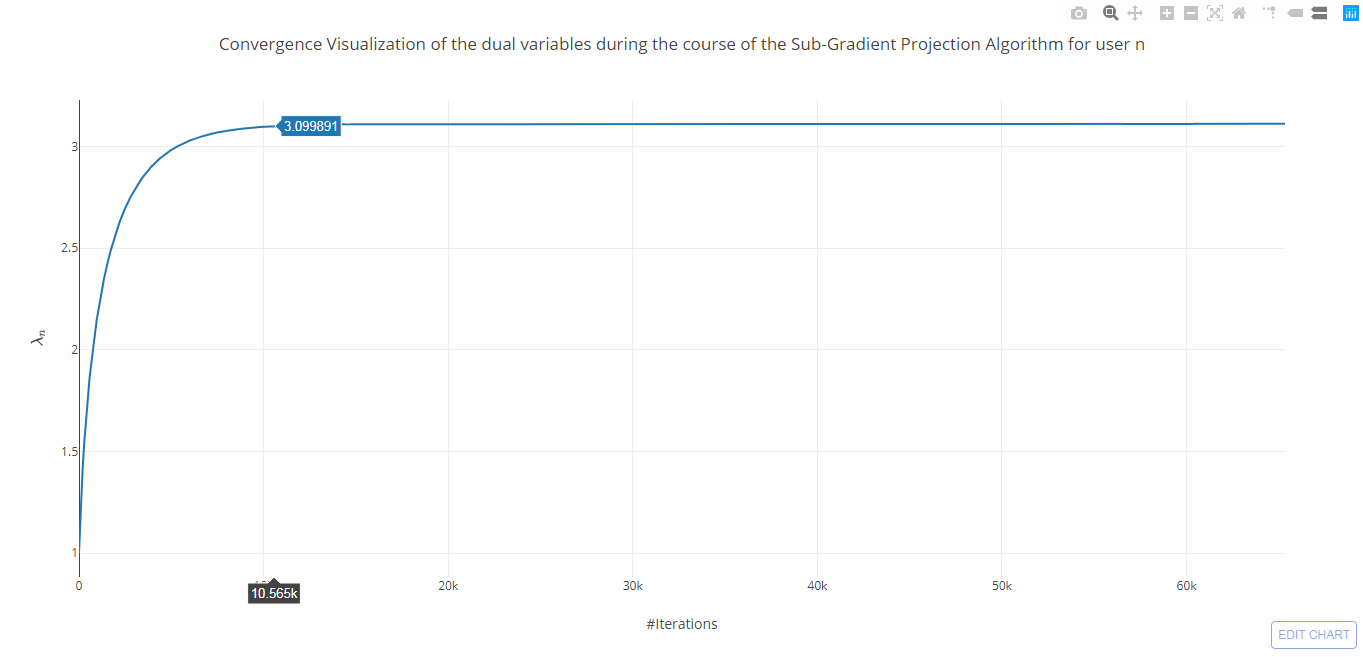
\includegraphics[width=1.0\textwidth]{Power_Allocation_Convergence_Analysis_Dual_Variables.png}
        \caption{Power Allocation Convergence Analysis for the Dual Variables using Sub-gradient Projection in the Dual}
        \label{fig:mesh1}
        \centering
    \end{figure}
    \item The MCS adaptation algorithm is:
    \begin{itemize}
        \item Upon receiving a packet, the SU node computes the SNR of the sub-link using MMSE estimation and knowing the modulation scheme and code rate used at the transmitter, the SU node calculates the PER.
        \item An exhaustive search (or a more optimal search, if possible) is performed over the set of MCS choices to determine their PER estimates. Then, choose an MCS such that,
        $MCS_{choice}=argmax_{MCS}\ r_{MCS}(1 - PER_{MCS})$
    \end{itemize}
    \item The algorithm derived for estimating the correlation model parameters is the Expectation-Maximization algorithm.
    \begin{figure}[t]
        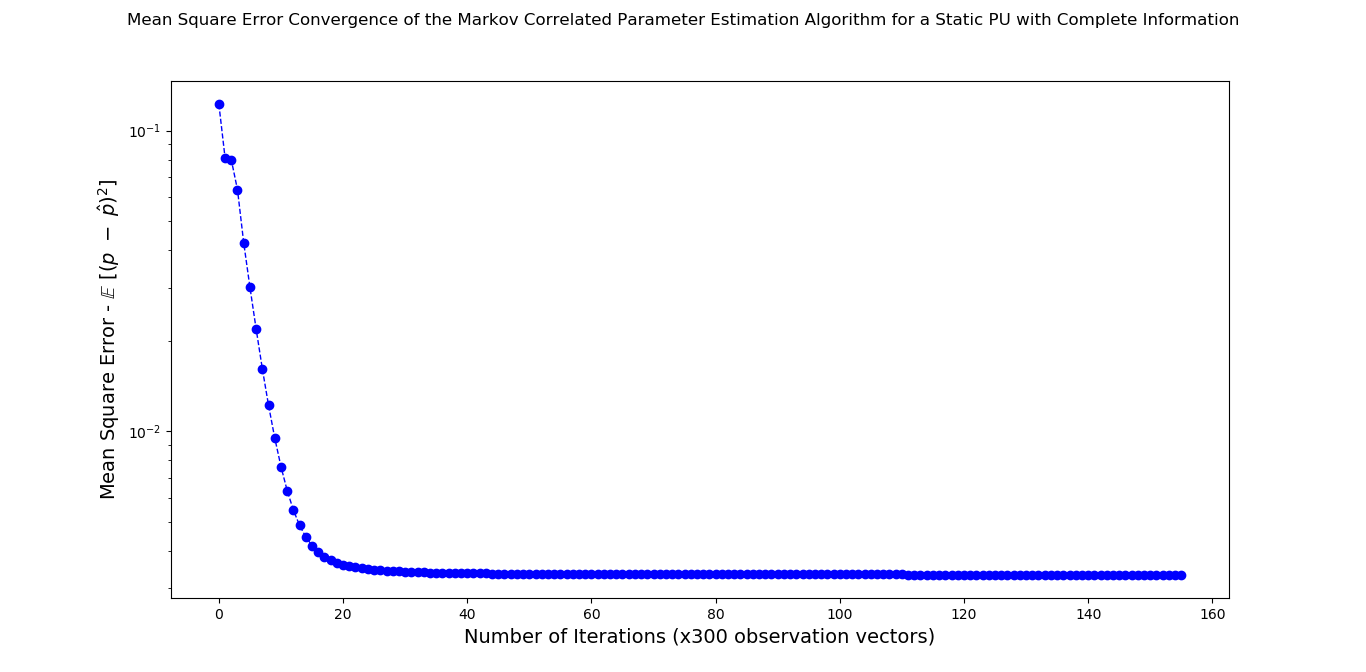
\includegraphics[width=1.0\textwidth]{Mean_Square_Plot_Log_Scale.png}
        \caption{Mean Square Error v/s Number of Iterations - A plot of convergence of our variant of EM for HMMs in order to estimate the parameters of the Markov Chain.}
        \label{fig:mesh2}
        \centering
    \end{figure}
    \item The algorithm derived for estimating the channel occupancy states from the HMM model (across channel indices and across time indices) is the Double-Markov Chain Viterbi algorithm.
    \item We employ the PERSEUS algorithm to solve for the optimal policy and based on this optimal policy we assign utility values to the channels in a given time-slot, disseminate this information over the control channel, and this utility information is captured in the back-up timer logic of the CSMA protocol running in the MAC layer.
    \begin{itemize}
    \item The PERSEUS Algorithm is a Randomized Approximate Point-Based Value Iteration Algorithm that involves the following steps:
    \begin{itemize}
        \item \textbf{Random Exploration}: In the exploration period, the POMDP agent randomly explores the radio environment and comes up with a set of "reachable beliefs" $B$.
        \item \textbf{Initialization}: All the elements in the initial value function $V_0$ are set to $\frac{1}{1-\gamma}min_{\vec{x},\ a}\ R(\vec{x},\ a)$.
        \item Arbitrarily, considering the $n$-th time-step, the \textbf{Backup} procedure involves the following,
        \begin{itemize}
            \item Initialize the set of unimproved belief points $\Tilde{B}\ =\ B$ and $V_{n+1}\ =\ \phi$
            \item Sample a belief point $\vec{b} \in \Tilde{B}$ uniformly at random and compute $\vec{\alpha}\ =\ backup(\vec{b})$
            \item If $\vec{b} \cdot \vec{\alpha} \geq V_n(\vec{b})$, then add $\vec{\alpha}$ to $V_{n+1}$, else add $\vec{\alpha}'\ =\ argmax_{\vec{\alpha}_n^i}\ \vec{b} \cdot \vec{\alpha}_n^i$ to $V_{n+1}$
            \item Remove all the improved points from $\Tilde{B}$, i.e. all the belief points $\vec{b} \in \Tilde{B}$ for which $\vec{b} \cdot \vec{\alpha} \geq V_n(\vec{b})$ are removed from $\Tilde{B}$
            \item Stop when $\Tilde{B}$ is empty
        \end{itemize}
        \item The backup steps are performed until the convergence condition is met, i.e. if the number of policy changes between $V_{n}$ and $V_{n+1}$ is less than a certain threshold $\eta$, we terminate the algorithm.
        \item An extension to the PERSEUS algorithm is to re-learn the set of "reachable beliefs" by allowing the POMDP agent to explore the radio environment with the most recent policy under the following circumstances:
        \begin{itemize}
            \item At the end of every $N$-th backup stage, or
            \item When the cumulative reward from the radio environment, i.e. a measure of the achieved throughput observed over a fixed period of time, drops below a certain threshold
        \end{itemize}
    \end{itemize}
    \begin{figure}[t]
        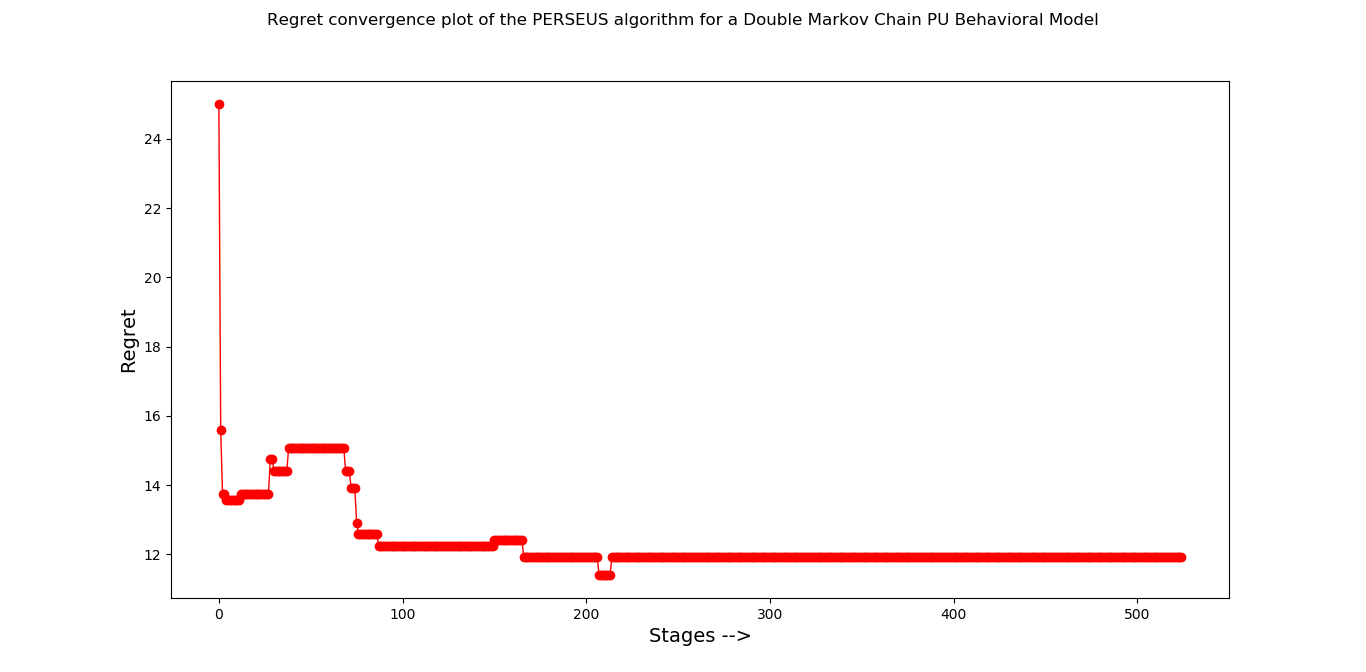
\includegraphics[width=1.0\textwidth]{Regret_Convergence_Plot_04112019.png}
        \caption{Regret Convergence plot of the PERSEUS algorithm while solving for the optimal policy}
        \label{fig:mesh3}
        \centering
    \end{figure}
    \begin{figure}[t]
        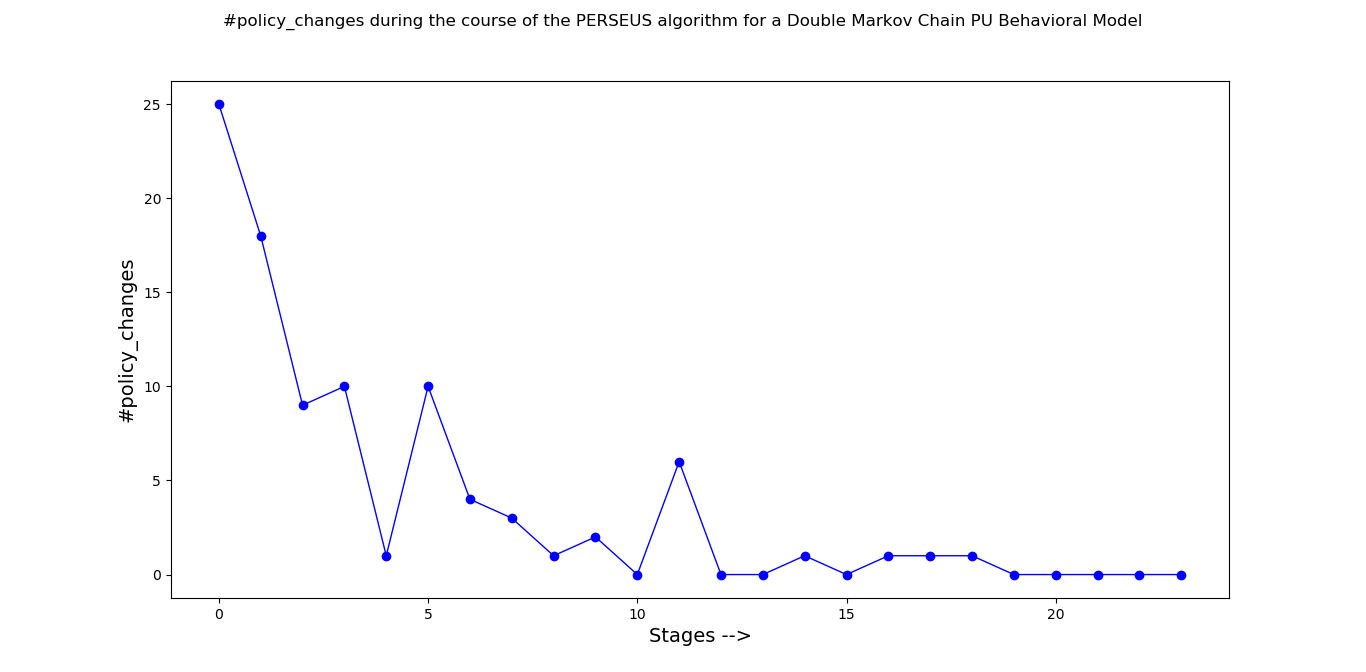
\includegraphics[width=1.0\textwidth]{Policy_Changes_Plot_04112019.png}
        \caption{Number of policy changes v Iteration index for the PERSEUS algorithm}
        \label{fig:mesh4}
        \centering
    \end{figure}
\end{itemize}
\end{itemize}
\clearpage
\section{Conclusion and Future Work}
\subsection{Conclusion}
\begin{itemize}
    \item We framed the cross-layer optimization problem as a Numerical Utility Maximization (NUM) formulation with constraints capturing protocol specifications from all five layers of the SU network protocol stack.
    \item Assuming a Markovian correlation model both spatially and temporally, we learn the model using a modified version of the Expectation-Maximization algorithm.
    \item Based on the noisy incomplete observations made at the SU spectrum sensors, we estimate the occupancy states using a extended version of the Viterbi algorithm and use these estimated states to evaluate the reward to the POMDP agent.
    \item The POMDP agent runs the PERSEUS algorithm (Approximate Point-Based Value Iteration over a reduced belief space) to get the optimal policy and the utility metrics obtained from this are employed in the CSMA algorithm's back-off timer logic.
    \item The cross-layer optimization problem is then solved for,
    \begin{itemize}
        \item Optimal Power Allocation - A variant of water-filling incorporating additional variables for occupancy indication and MRR requirements from the application layer
        \item MCS adaptation - Receiver-based MCS adaptation, SNR and PER estimation; choose an MCS from the set of available MCS choices that maximizes $r_{MCS}(1 - PER_{MCS})$
        \item Flow Routing - Inverse utility function of the length of the Injected\_Pending\_Queue for every flow $f \in \mathcal{F}$
        \item Prioritized Flow Scheduling - Weighted queue differential back-pressure scheduler
        \item Channel Access - CSMA at the MAC layer with transmission aggressiveness governed by the channel availability metrics obtained from the POMDP agent (gateway node) over the control channel and the queue back-pressure on the link.
    \end{itemize}
\end{itemize}
\subsection{Future Work}
There is the problem of System Dynamics involved in the POMDP formulation. Since there are a lot of moving parts to the radio environment we're operating in, recent research detailed in ``\href{https://ieeexplore.ieee.org/document/8303773}{\textcolor{blue}{Deep Reinforcement Learning for Dynamic Multi-channel Access in Wireless Networks}}" and ``\href{https://arxiv.org/pdf/1109.2145.pdf}{\textcolor{blue}{Perseus: Randomized Point-based Value Iteration for POMDPs}}" suggest that Re-Learning OR Re-Training gives us significantly better performance than our current approach of operating a reactive strategy.
\\For instance, a proactive strategy with re-training is shown to be an effective solution as opposed to a Reactive Whittle-Index based strategy in ``\href{https://ieeexplore.ieee.org/document/8303773}{\textcolor{blue}{Deep Reinforcement Learning for Dynamic Multi-channel Access in Wireless Networks}}". We can take two approaches to re-training:
\begin{itemize}
    \item We can develop extensions to the work outlined in ``\href{https://arxiv.org/pdf/1109.2145.pdf}{\textcolor{blue}{Perseus: Randomized Point-based Value Iteration for POMDPs}}" in order to re-learn the most relevant belief states and then use those in our Approximate Value Iteration Algorithm to solve for an optimal policy.
    \begin{itemize}
        \item We can re-sample the set of reachable belief points using our most recent policy when the accumulated reward experiences a significant drop.
        \item We can then use this new set of reachable belief points to solve for a new optimal policy using the PERSEUS algorithm ("Backup" until all belief points in the reachable set have been sampled and Update the Value Function for these beliefs based on the chosen policy tree vector).
    \end{itemize}
    \item Another possible approach would be to employ Adaptive Deep Q-Networks. Adaptive DQNs turn out to be great tools to solve for an optimal policy in highly-dynamic environments where the system statistics are unknown.
    \begin{itemize}
        \item Reference ``\href{https://ieeexplore.ieee.org/document/8303773}{\textcolor{blue}{Deep Reinforcement Learning for Dynamic Multi-channel Access in Wireless Networks}}" uses the Deep Q-Learning with Experience Replay Algorithm to design the DQN.
        \begin{itemize}
            \item Design: 2-layer Neural Network with 200 neurons and a ReLU activation function at each neuron
            \item An $\epsilon$-greedy policy is employed to select actions (channel combinations) in a given state. The interaction record - \textit{(state, action, observation, reward, next-state)} is stored in a "Replay Memory" and a random set of these historic records are used to compute the loss function.
            \item The weights of the DQN are updated using the stochastic gradient-descent algorithm
        \end{itemize}
        \item This DQN is used in conjunction with a re-training policy which involves evaluation of the accumulated reward of the current policy and simply comparing it with a threshold in order to trigger re-training to find a new good policy.
    \end{itemize}
\end{itemize}
\end{document}